\section{Maintaining and contributing to a forked repository\label{sec:maintain_repo}}

This section covers the following details

\begin{enumerate}
	\item Checking the status of the forked repository compared to the master repository
	\item Updating forked repository
	\item Making changes to your forked repository
\end{enumerate}

\subsection{Checking the status of the forked repository}

The status of the forked repository as compared to the master repository can be seen on github ()see Figure~\ref{fig:fork_status})

\begin{figure}[!ht]
	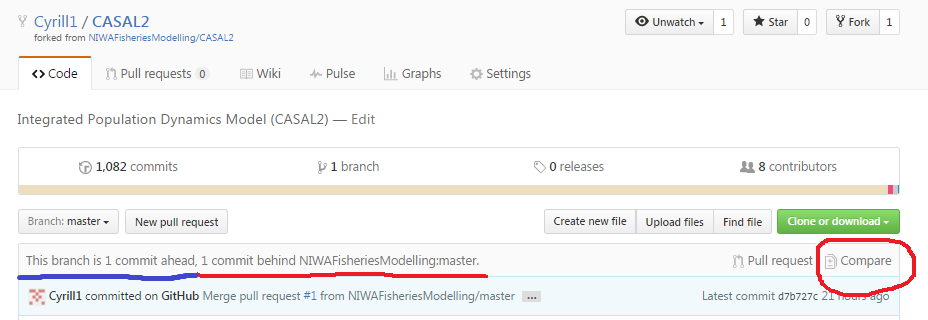
\includegraphics[scale=0.6]{Figures/fork_status.png}
	\caption{Fork status}\label{fig:fork_status}
\end{figure}

This line underlined in red indicates the relationship between the master and the forked version. In the above example, the forked version is one commit behind the master. 

To update this forked repository, click the `compare' button (circled in red on the right of the above example figure). This will bring up a page that will tell you of the changes that have occurred to the master repository. 

There are two situations that can occur when updating a forked repository. The first and easiest is that there is no conflicts and you can merge the master changes with ease, the second is there are conflicts. The second case is described below.

\subsection{Updating the forked repository}

Craig to add a section here.
